\documentclass[a4paper,12pt]{article}

\usepackage[14pt]{extsizes}
\usepackage{cmap}					% поиск в PDF
\usepackage{mathtext} 				% русские буквы в формулах
\usepackage[T2A]{fontenc}			% кодировка
\usepackage[utf8]{inputenc}			% кодировка исходного текста
\usepackage[english,russian]{babel}	% локализация и переносы
\usepackage{graphicx}
\usepackage{geometry}
\usepackage{amsmath}
\usepackage{amssymb}
\usepackage[table]{xcolor}
\setlength\extrarowheight{2pt}
\usepackage{multirow}


\geometry{verbose, a4paper, tmargin=2cm, bmargin=2cm, lmargin=3cm, rmargin=2cm}
\author{Vysotsky Maxim}
\title{Отчёт}
\date{2024}

\begin{document}
	\begin{titlepage}
		\begin{center}
			{Министерство науки и высшего образования Российской Федерации
				НОВОСИБИРСКИЙ НАЦИОНАЛЬНЫЙ ИССЛЕДОВАТЕЛЬСКИЙ
				ГОСУДАРСТВЕННЫЙ УНИВЕРСИТЕТ (НГУ)}
		\end{center}
		\begin{center}
			{Физический факультет}
		\end{center}
		\begin{center}
			{Кафедра общей физики}
		\end{center}
		
		
		\vspace{7cm}
		{
			\begin{center}
				{\bf Лабораторная работа №1.1}\\
				Измерение стационарных случайных величин и статистическая обработка результатов измерений
			\end{center}
		}
		\vspace{2cm}
		\begin{flushright}
			{Руководитель:\\ Старший преподаватель\\
				Яцких А. А.\\
				Работу выполнил:\\
				Высоцкий М. Ю.\\
				\vspace{0.2cm}
				гр. 24301}
		\end{flushright}
		\vspace{3cm}
		\begin{center}
			Новосибирск, 2024
		\end{center}
	\end{titlepage}

\section{Теоретическое введение}
\textbf{Цель работы:} Ознакомление с методами обработки и представления
результатов измерений случайных величин на примере исследования ин-
тенсивности излучения $\alpha$-частиц при радиоактивном распаде ядер.
В данной лабораторной работе исследуется интенсивность изотопного
источника $\alpha$-частиц (измеряется количество n $\alpha$-частиц, испускаемых ис-
точником за фиксированный промежуток времени $\tau$).

\textbf{Оборудование:} Оборудование представлено на рисунке снизу.
\begin{figure}[ht!]
    \centering
    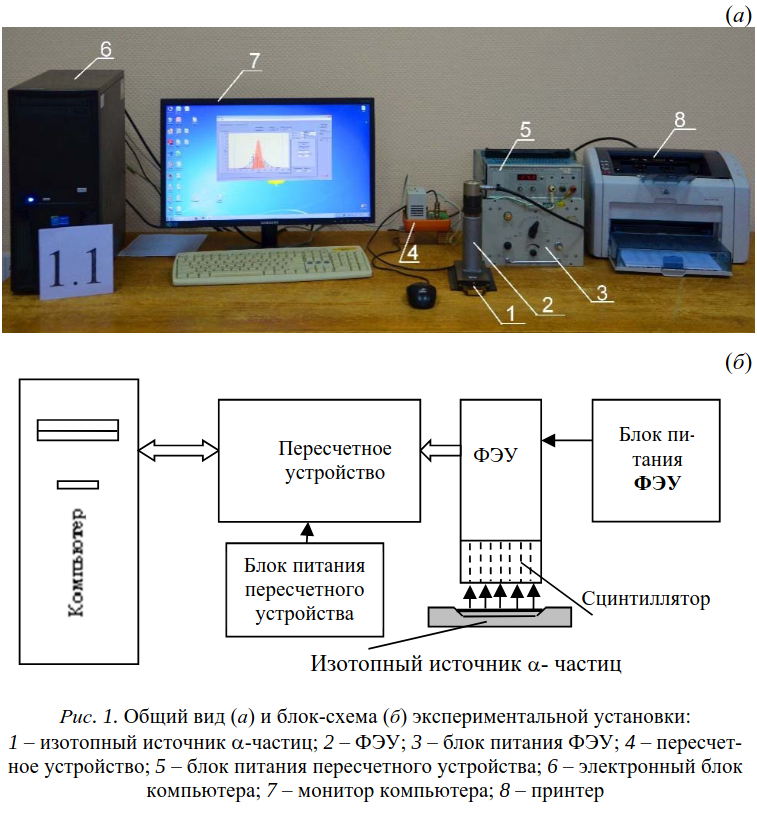
\includegraphics[scale=0.7]{scheme_1.png}
    \caption{Установка}
\end{figure}

\newpage
\section{Ход работы}
\subsection{Задание 1. Счетная характеристика детектора}
\hspace{\parindent} В данном задании требуется провести серию экспериментов с источником $\alpha$-излучения и без него (для определения вклада теневого тока). Производится серия измерений от 1,2 кВ до 2,5 кВ с шагом в 0,1 кВ, снимается показание $\overline{x}$ и $S_n$. Берём интервал измерений $\Delta$ T = 200 мсек и число измерений N = 50 шт. Данные приведены ниже.

\begin{table}[!ht]
    \centering
    \begin{tabular}{|l|l|l|}
    \hline
        $U$, В & $\overline{x}$ & $S_n$ \\ \hline
        1,20 & 11,20 & 3,150 \\ \hline
        1,30 & 10,42 & 2,984 \\ \hline
        1,40 & 10,22 & 3,340 \\ \hline
        1,50 & 210,58 & 13,720 \\ \hline
        1,60 & 275,96 & 16,536 \\ \hline
        1,70 & 290,78 & 19,632 \\ \hline
        1,80 & 297,86 & 17,778 \\ \hline
        1,90 & 328,98 & 18,230 \\ \hline
        2,00 & 449,86 & 23,762 \\ \hline
        2,10 & 915,06 & 36,335 \\ \hline
        2,20 & 1808,14 & 66,223 \\ \hline
        2,30 & 2650,10 & 105,052 \\ \hline
        2,40 & 3384,02 & 125,086 \\ \hline
        2,50 & 4055,26 & 236,540 \\ \hline
    \end{tabular}
    \caption{Данные с источником $\alpha$-излучения.}
\end{table}

\begin{table}[!ht]
    \centering
    \begin{tabular}{|l|l|l|}
    \hline
        $U$, В & $\overline{x}$ & $S_n$ \\ \hline
        1,2 & 0,00 & 0,00 \\ \hline
        1,3 & 0,02 & 0,14 \\ \hline
        1,4 & 0,02 & 0,14 \\ \hline
        1,5 & 0,04 & 0,20 \\ \hline
        1,6 & 0,48 & 0,58 \\ \hline
        1,7 & 1,06 & 1,13 \\ \hline
        1,8 & 4,78 & 1,94 \\ \hline
        1,9 & 27,04 & 4,45 \\ \hline
        2,0 & 166,74 & 14,72 \\ \hline
        2,1 & 523,32 & 22,51 \\ \hline
        2,2 & 905,58 & 90,71 \\ \hline
        2,3 & 1253,58 & 39,10 \\ \hline
        2,4 & 1811,92 & 66,19 \\ \hline
        2,5 & 2029,56 & 52,81 \\ \hline
    \end{tabular}
    \caption{Данные без источника $\alpha$-излучения.}
\end{table}

\clearpage  
Графики $\overline{x}(U)$ и $\overline{x_т}(U)$ приведены далее.
\begin{figure}[ht!]
    \centering
    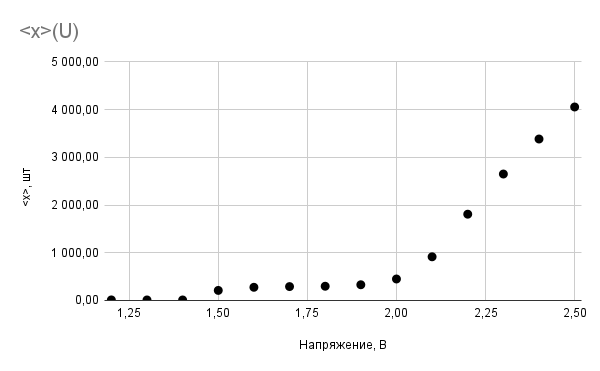
\includegraphics[scale=0.7]{xu.png}
    \caption{Зависимость $\overline{x}(U)$}
\end{figure}

\begin{figure}[ht!]
    \centering
    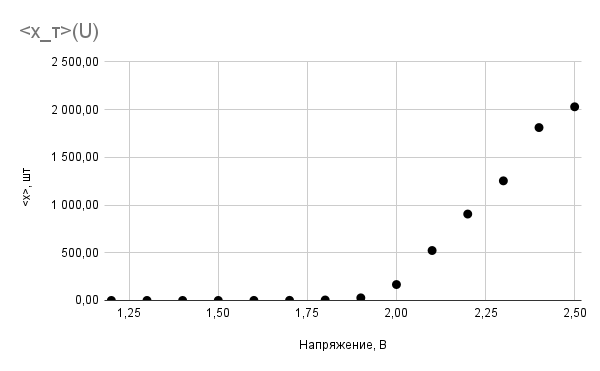
\includegraphics[scale=0.7]{xtu.png}
    \caption{Зависимость $\overline{x_т}(U)$}
\end{figure}

\clearpage
Для оценки систематической погрешности воспользуемся формулой:
\begin{equation}
    \frac{\overline{x_т}}{\overline{x}} * 100\%
\end{equation}

Получаем следующие значения:

\begin{table}[!ht]
    \centering
    \begin{tabular}{|l|l|l|l|}
    \hline
        $U$, кВ & $\overline{x}$ & $\overline{x_т}$ &  $\overline{x_т}/{\overline{x}}, \% $\\ \hline
        1,2 & 11,20 & 0,00 & 0 \\ \hline
        1,3 & 10,42 & 0,02 & 0,19 \\ \hline
        1,4 & 10,22 & 0,02 & 0,2 \\ \hline
        1,5 & 210,58 & 0,04 & 0,02 \\ \hline
        1,6 & 275,96 & 0,48 & 0,17 \\ \hline
        1,7 & 290,78 & 1,06 & 0,36 \\ \hline
        1,8 & 297,86 & 4,78 & 1,6 \\ \hline
        1,9 & 328,98 & 27,04 & 8,22 \\ \hline
        2,0 & 449,86 & 166,74 & 37,06 \\ \hline
        2,1 & 915,06 & 523,32 & 57,19 \\ \hline
        2,2 & 1808,14 & 905,58 & 50,08 \\ \hline
        2,3 & 2650,10 & 1253,58 & 47,3 \\ \hline
        2,4 & 3384,02 & 1811,92 & 53,54 \\ \hline
        2,5 & 4055,26 & 2029,56 & 50,05 \\ \hline
    \end{tabular}
    \caption{Отношение $\overline{x_т}/{\overline{x}}$}
    \label{xtx}
\end{table}

Из таблицы (\ref{xtx}) можно сделать вывод о том, что теневой ток ФЭУ оказывает малое влияение на показания в диапазоне от 1,2 кВ до 1,8 кВ. Далее влияение растёт вплоть до $\approx 57\%$. 

\clearpage

\subsection{Задание 2. Влияние числа измерений и интервала счета
на точность определения среднего}
\hspace{\parindent} В данном задании нужно провести измерения при разных интервалах и проследить изменение СОС, СКО в зависимости от числа измерений.


\begin{figure}[ht!]
    \centering
    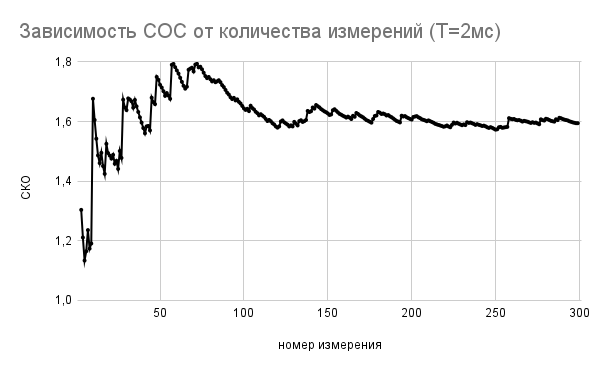
\includegraphics[scale=0.7]{sos2.png}
    \caption{Зависимость СОС от количества измерений при $\Delta$ T = 2 мс}
\end{figure}

\begin{figure}[ht!]
    \centering
    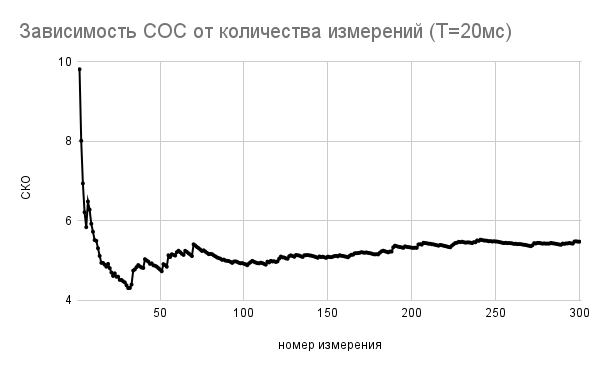
\includegraphics[scale=0.7]{sos20.png}
    \caption{Зависимость СОС от количества измерений при $\Delta$ T = 20 мс}
\end{figure}

\begin{figure}[ht!]
    \centering
    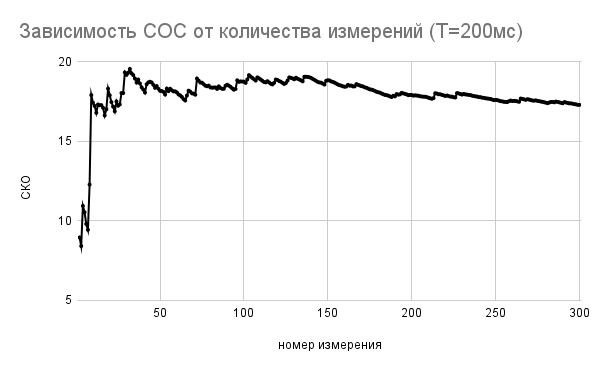
\includegraphics[scale=0.7]{sos200.png}
    \caption{Зависимость СОС от количества измерений при $\Delta$ T = 200 мс}
\end{figure}

Переведя значения в \textit{распады в секунды}, найдя средние значения и погрешности, мы получаем:\\
Для 2 мс:
\begin{equation}
    1443 \pm 46 \pm 5 \hspace{7pt} расп/с
\end{equation}
Для 20 мс:
\begin{equation}
    1512 \pm 16 \pm 5 \hspace{7pt} расп/с
\end{equation}
Для 200 мс:
\begin{equation}
    1506 \pm 5 \pm 5 \hspace{7pt} расп/с
\end{equation}

\subsection{Вывод по заданию}
\hspace{\parindent}Здесь я делаю вывод, что при большем интервале измерений мы получаем меньшую статистическую погрешность (что видно и из графиков), потому мы получаем очевидный критерий: больше интервал измерений - меньше стат. погрешность.

Также из графиков видно оптимальное количество измерений, когда СКО выравнивается:\\
Для 2 мс: 150-175 измерений.\\
Для 20 мс: 75-100 измерений.\\
Для 200 мс: 75-100 измерений.

\clearpage
\subsection{Задание 3. Идентификация аналитической модели
закона распределения}
\centering\Large \textbf{Смотрим фоточки}\\
\small шпингалеты лопнули




\end{document}
